% The document class marks this as a poster, supplying various options that
% control rendering of some standard features (e.g., the title bar).

\documentclass[ % the name of the author
                    author={Liam O'Shea},
                % the name of the supervisor (preferably including title)
                supervisor={Dr. Sion Hannuna},
                % the thesis    title (which cannot be blank)
                     title={ZeroToHero},
                % the thesis subtitle (which can    be blank)
                  subtitle={},
                % the degree programme (from BSc, MEng, MSci, MSc and PhD)
                    degree={Bsc},
                % the year of submission
                      year={2014} ]{poster}

\usepackage{epstopdf}
\usepackage{algorithm2e}
\begin{document}

% -----------------------------------------------------------------------------

\begin{frame}{} 

\vfill

\begin{columns}[t]
    \begin{column}{0.900\linewidth}
    \begin{block}{\normalsize Introduction}
    \small Computer aided coaching has revolutionised training approaches and been a key driver
            in improving sports performance at the highest level. Professional athletes can now use
            advanced augmented coaching to accurately and reliably measure a range of metrics that
            are then used as indicators of performance. ZeroToHero implements punch classification \& qualitative assessment of boxing pose and technique using the Kinect, a low cost consumer device that can bring specialist boxing coaching to everyone.{\newline}
            This research is borne out of a desire to improve access and cost to boxing coaching which are problems I have encountered first hand through the University Boxing Club. In the wider environment It could be used in developing countries where physical access to coaches with the
            required expertise may be difficult as well as local clubs in the UK.

    \end{block}
    \end{column}
\end{columns}

\vfill

\begin{columns}[t]
    \begin{column}{0.422\linewidth}
    \begin{block}{\normalsize 1. Dimensionality Reduction}
    \small Sets of data were recorded from local boxers, university
        boxers and professional boxers to `'ground-truth'' my data.
        Both linear and manifold learning techniques were tested to compare their effectiveness at producing usefully reduced data. 
    \begin{figure}[h]
        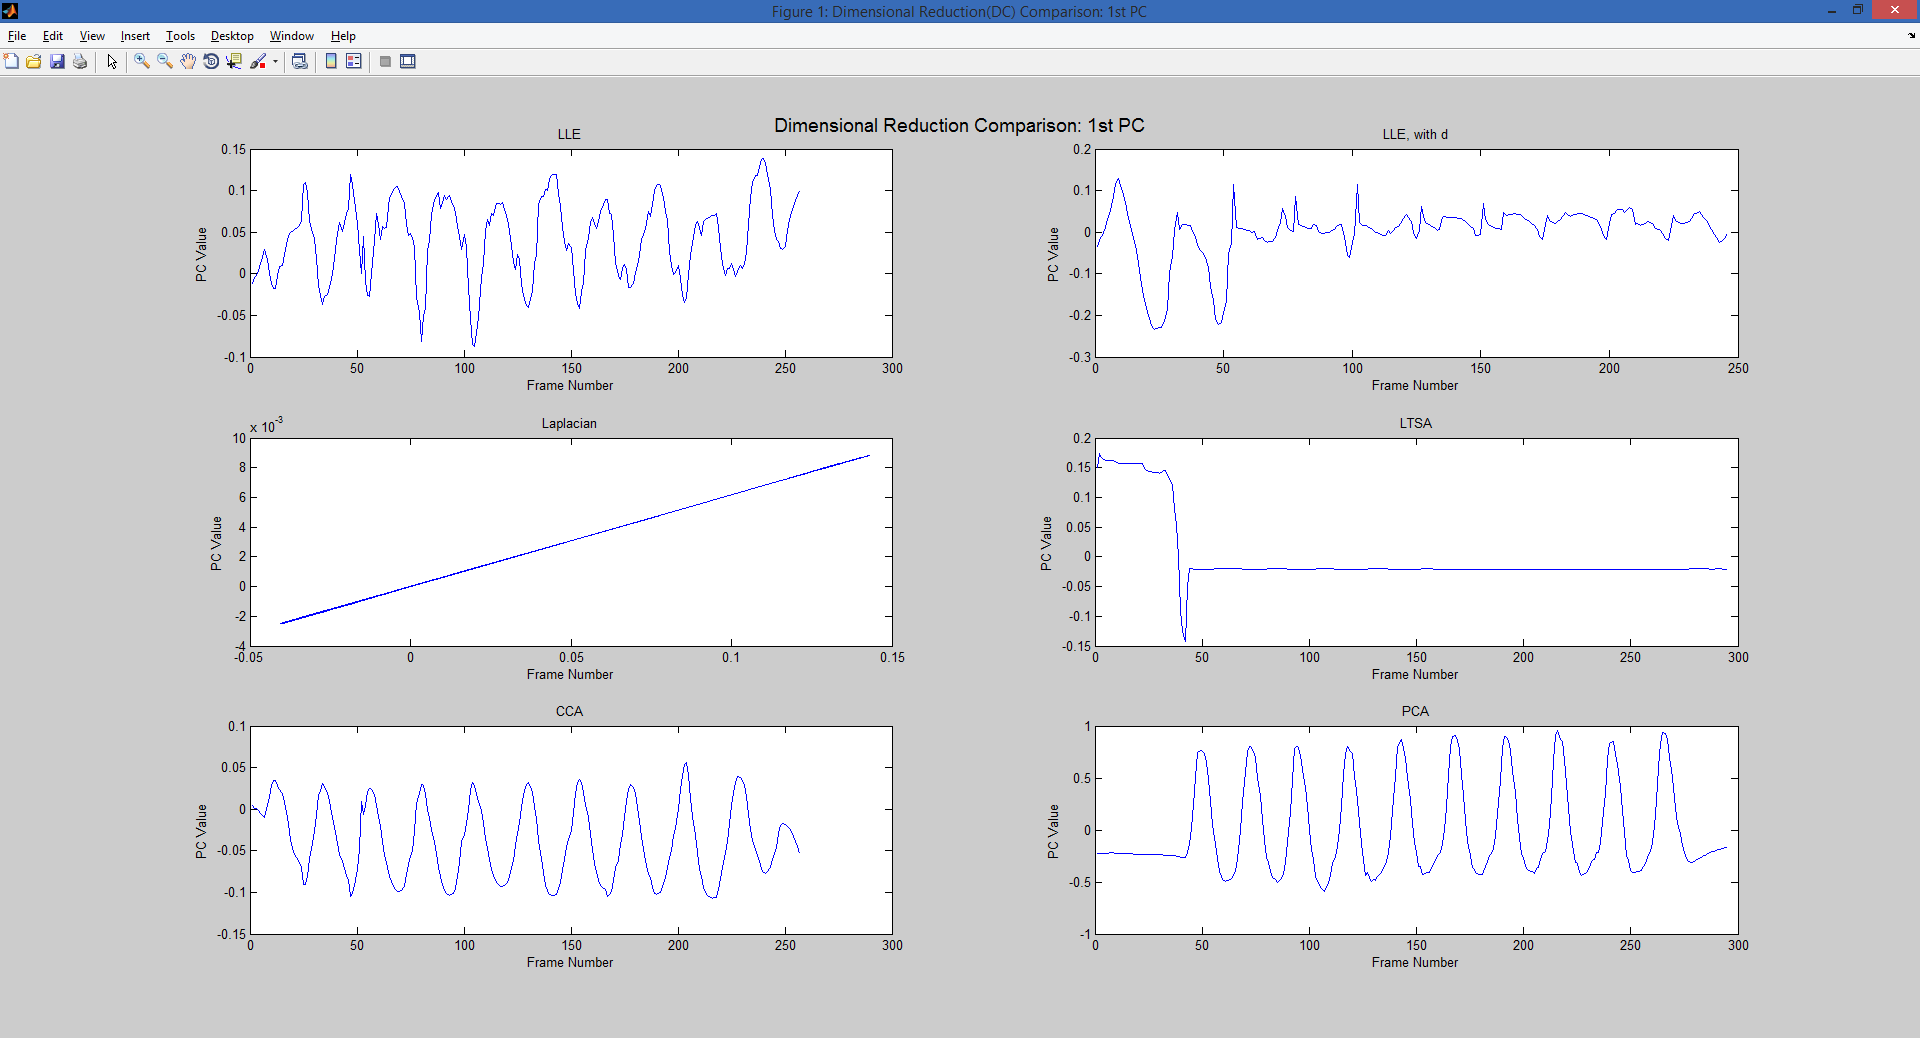
\includegraphics[height=0.20\textheight]{images/drcomp}
    \end{figure}
        Diffusion Maps \& Hidden Markov Models were also looked at but as shown above, PCA produced the most useful periodic time series. Due to
         it's linearity it also allowed my to project back and reconstruct my original and check for error. 
    \end{block}
    \end{column}

    \begin{column}{0.422\linewidth}
    \begin{block}{\normalsize 2. Punch Segmentation}
    \small Skeleton data was recorded from local boxers, university boxers and professional boxers whilst performing punches to `ground-truth' my data. Dimensionality reduction was performed on the raw data before using a set of heuristic rules to find the beginning of each punch.
    Evenly spaced samples are taken from each punch and used as a set of features for that type of punch.

    % \begin{figure}[h]
    % \begin{flushright}
    %     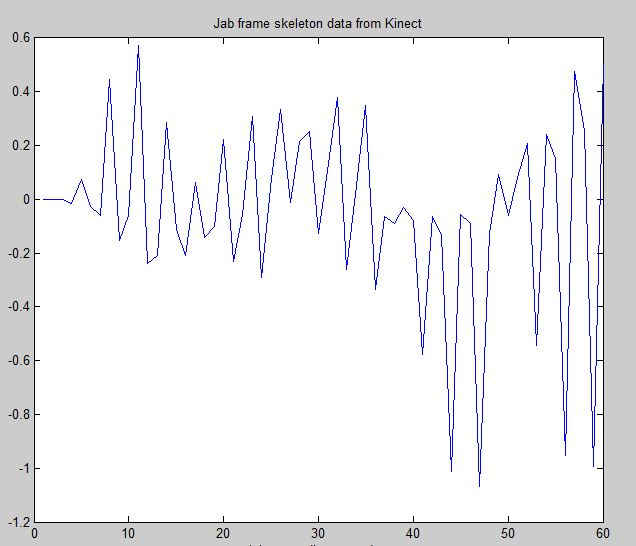
\includegraphics[height=0.10\textheight]{images/initjab}
    
    % \end{flushright}
    % \end{figure}

    \begin{figure}[h]
        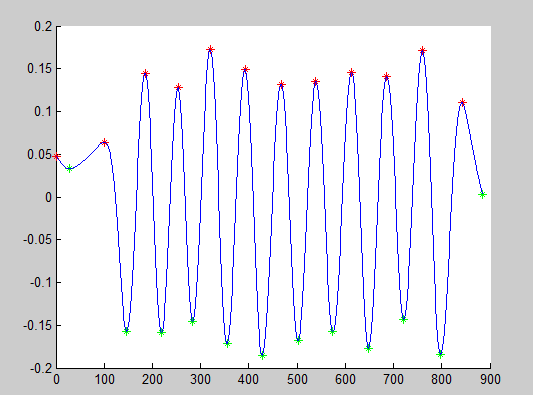
\includegraphics[height=0.10\textheight]{images/jabseg}
        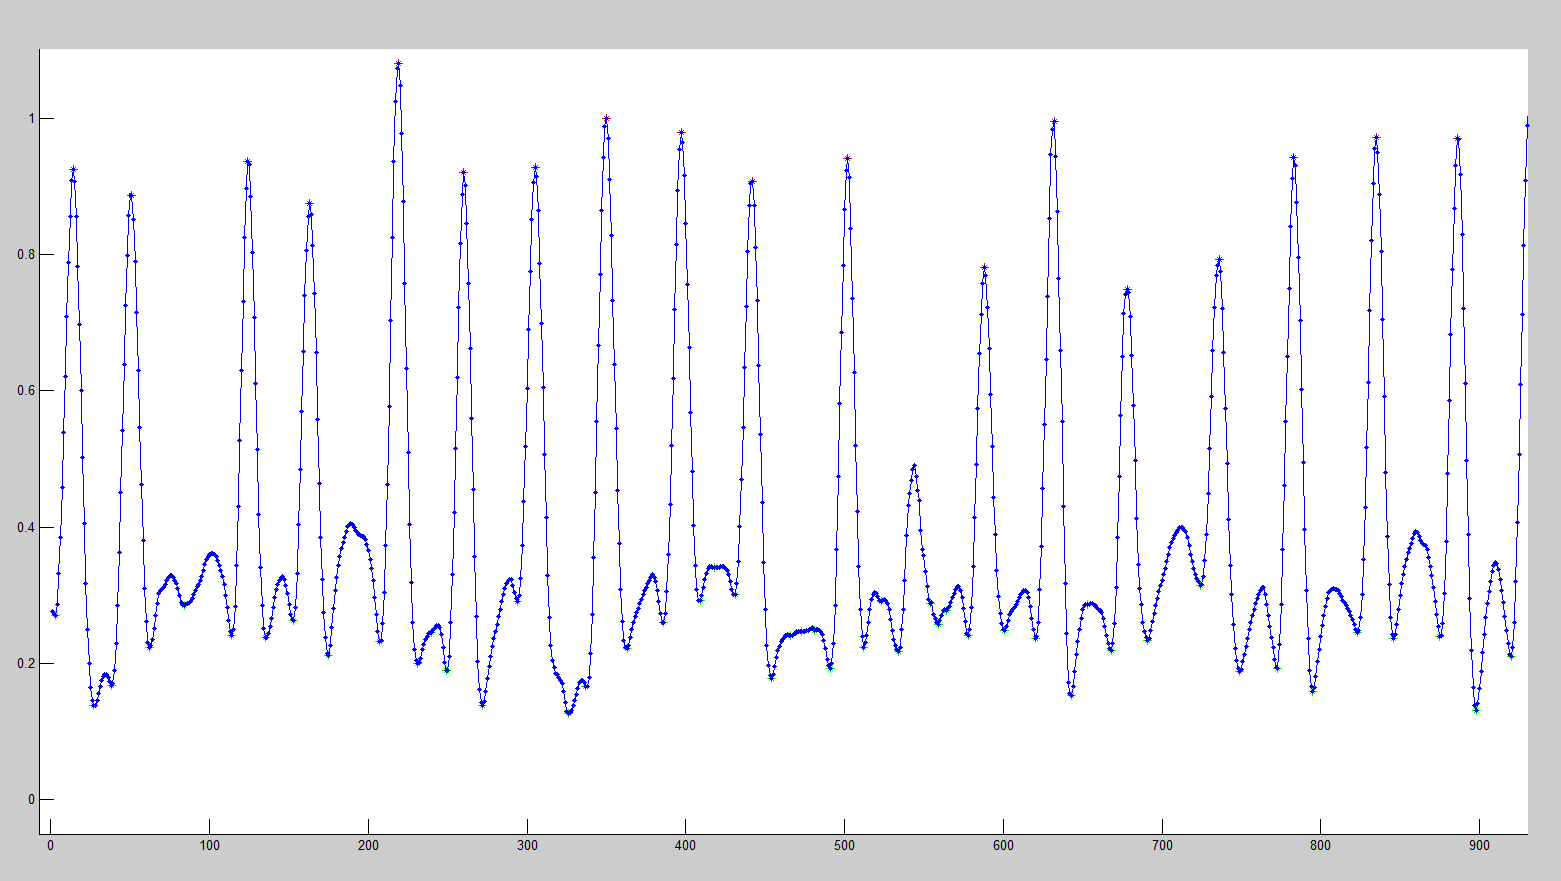
\includegraphics[height=0.10\textheight]{images/crossseg}
    \end{figure}

    \begin{figure}[h]
        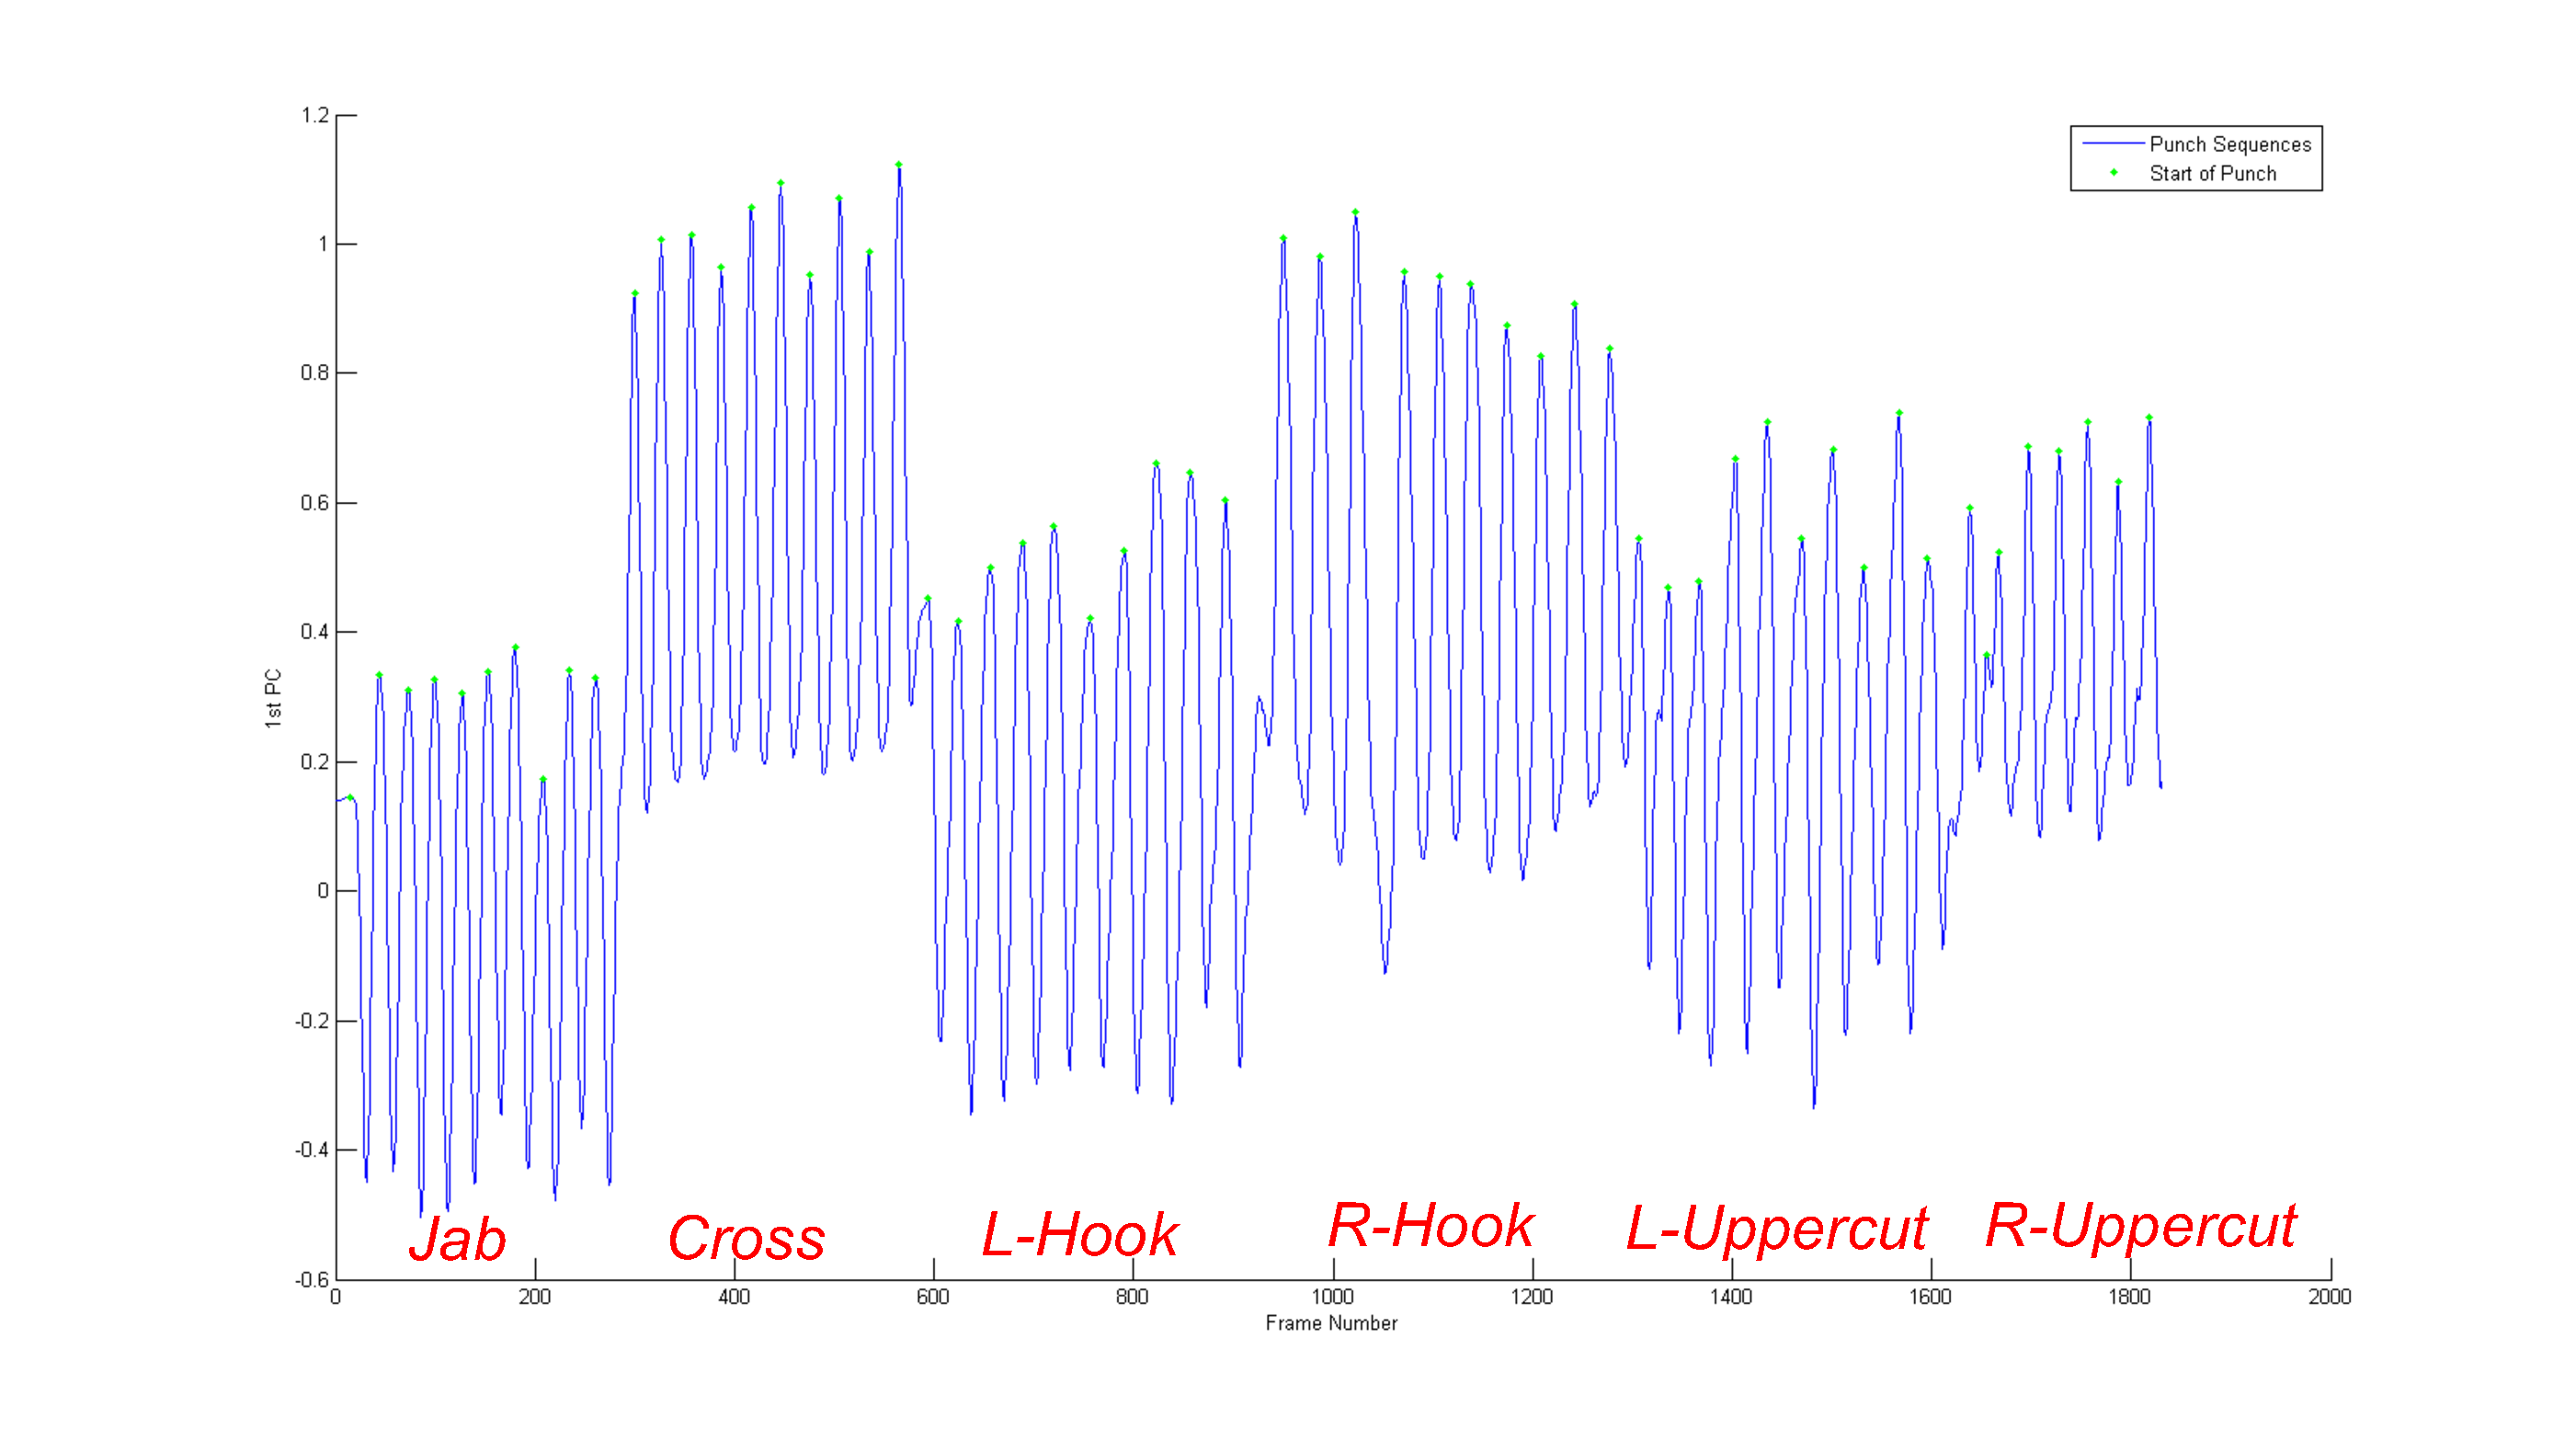
\includegraphics[height=0.15\textheight, width=0.35\textheight]{images/punchseq-pdf}
    \end{figure}
    \end{block}
    \end{column}
\end{columns}




%\vfill

\begin{columns}[t]
    \begin{column}{0.422\linewidth}
    \begin{block}{\normalsize 3. Classification}
    \small  After segmentation a variety of classification methods such as Dynamic Time Warping, FFT, Decision Trees, multi class Support Vector Machines \&  Neural Networks were trialled.
    \vspace{2.00mm}
    \begin{figure}[h]
        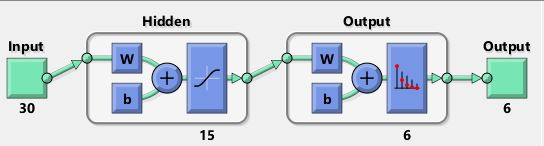
\includegraphics[width=0.28\textheight]{images/neuralnet}
    \end{figure}
    \begin{figure}[h]
        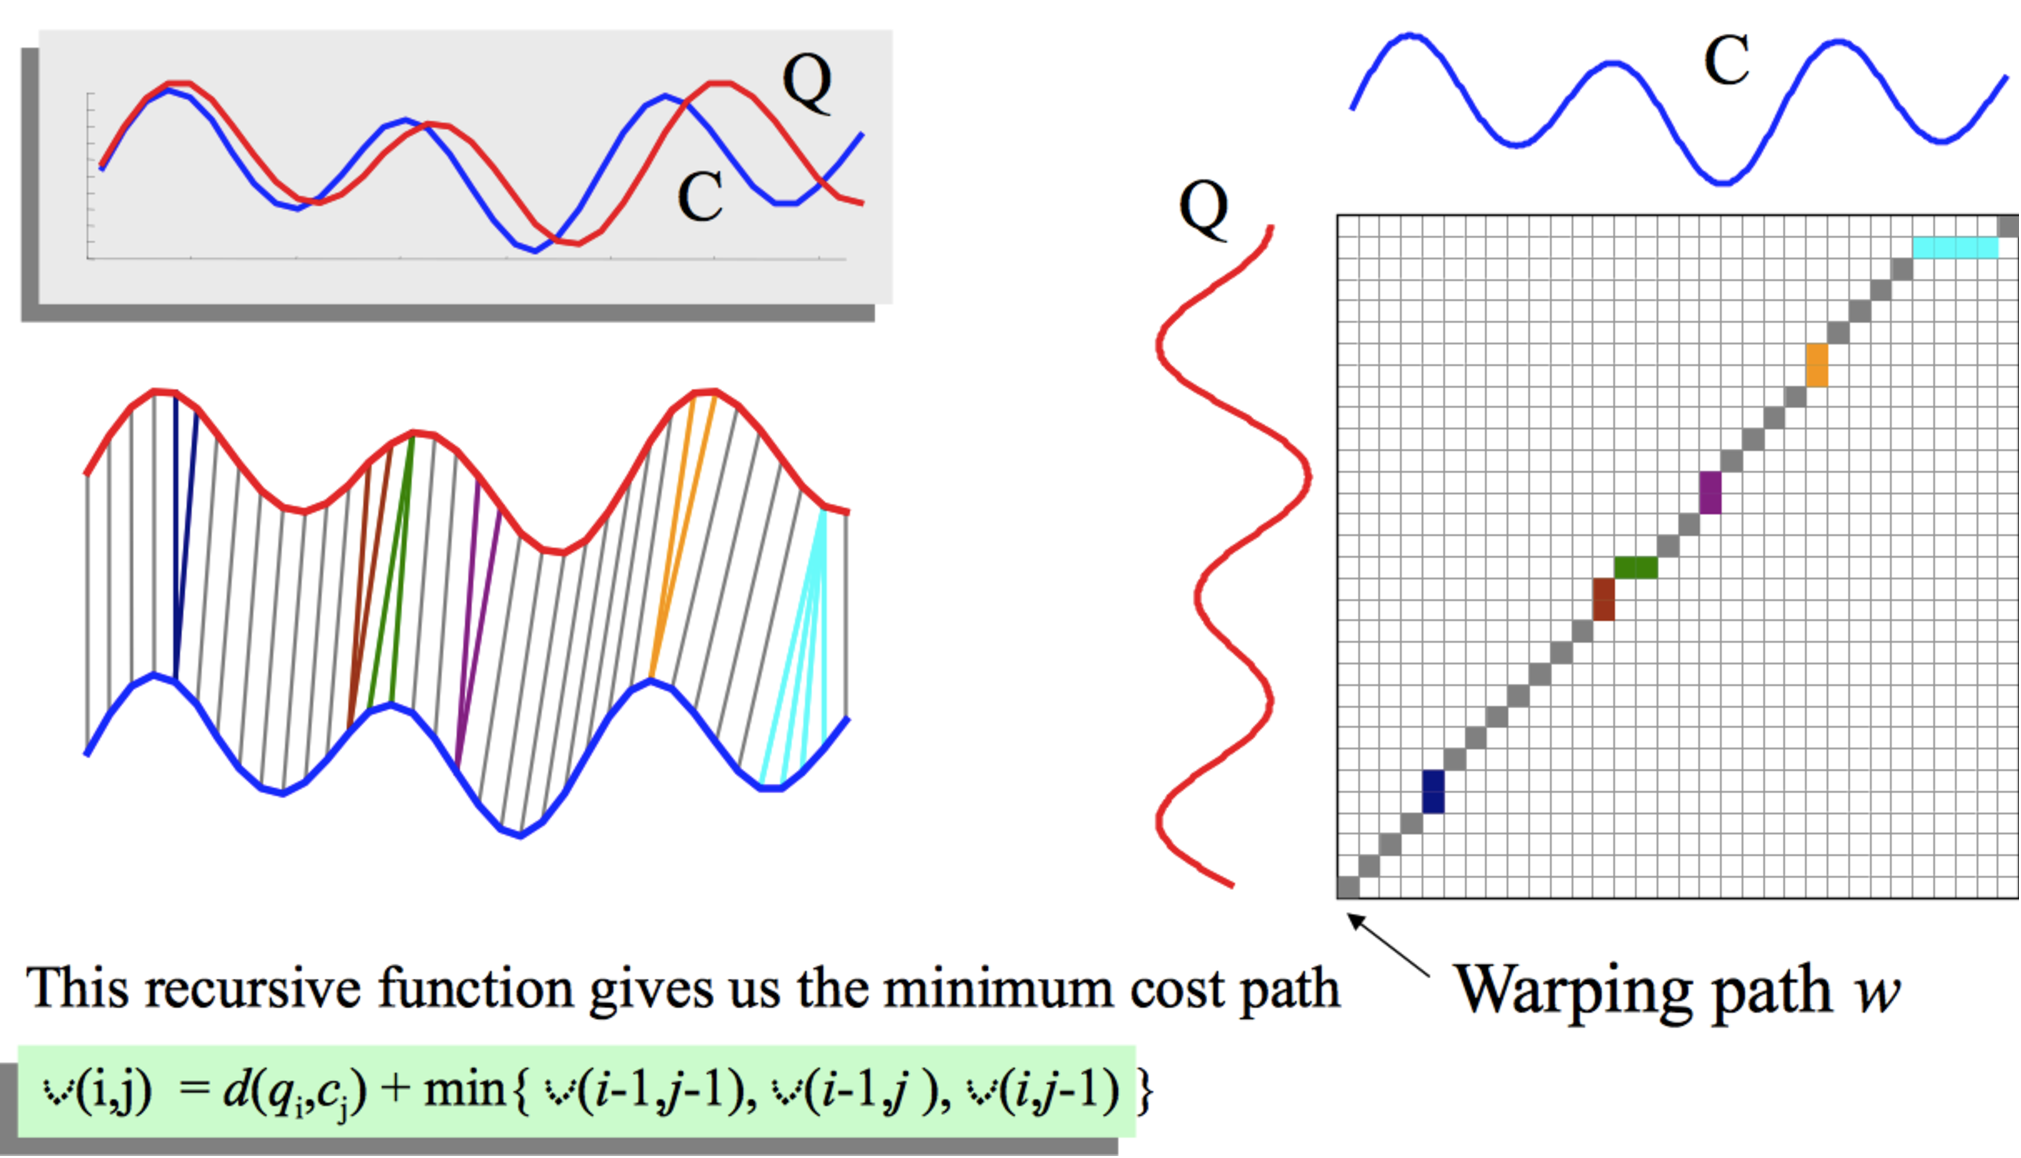
\includegraphics[height=0.15\textheight, width=0.30\textheight]{images/dtw-pdf.pdf}
    \end{figure}   
    \end{block}
    \end{column}
    
    \begin{column}{0.422\linewidth}
    \begin{block}{\normalsize 4. Results}
    \small When classifying a series of mixed punches a score of \boldmath{$85\%-93\%$} is achieved. On a two-class problem such as `'good jabs vs bad jabs'' a \textbf{99\%} detection rate has been achieved.
    \vspace{2.00mm}
    \begin{figure}[h]
        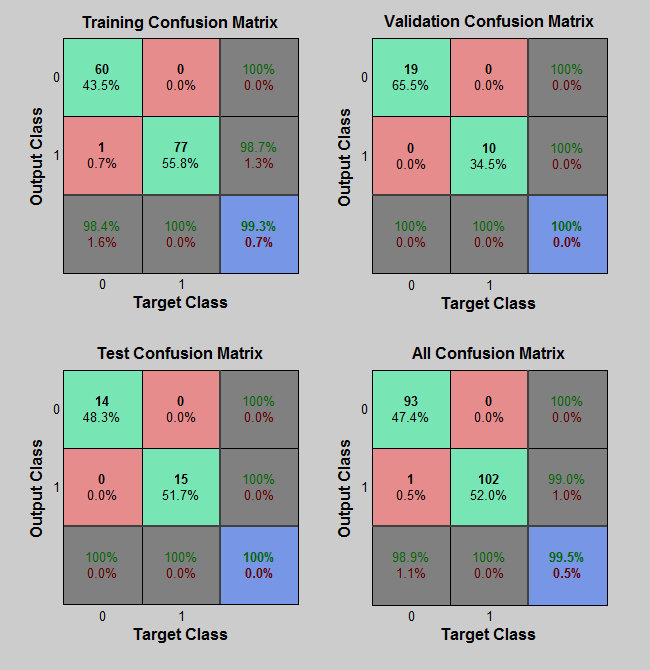
\includegraphics[height=0.15\textheight]{images/confm2}
        \vspace{1.00mm}
        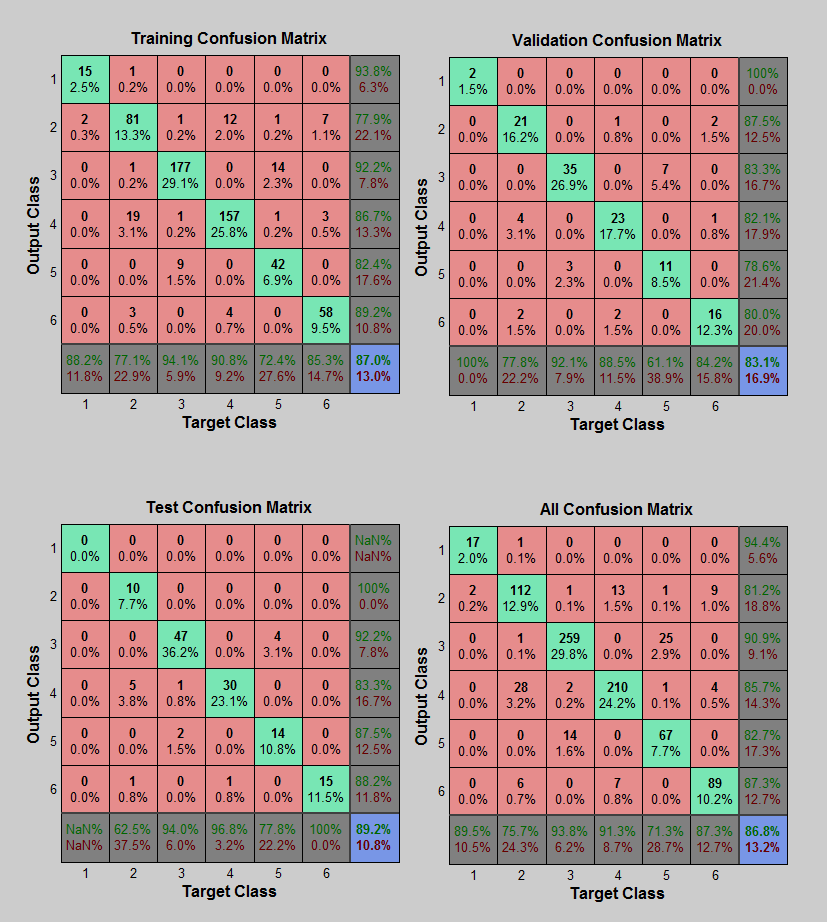
\includegraphics[height=0.15\textheight]{images/confm6}
    \end{figure}
    \end{block}
    \end{column}
\end{columns}

\vfill

\end{frame}

% -----------------------------------------------------------------------------

\end{document}



